\section{Appendix: Preliminary Models for State-of-the-Art NLP Algorithms} \label{app:Appendix_BasicsRNNLSTM}

\subsection{Recurrent Neural Networks (RNN)} \label{sec:RNN}


\subsubsection{Motivation for RNNs}

{
\begin{wrapfigure}{L}{0.6\textwidth}
\begin{center}
    \vspace{-20pt}
    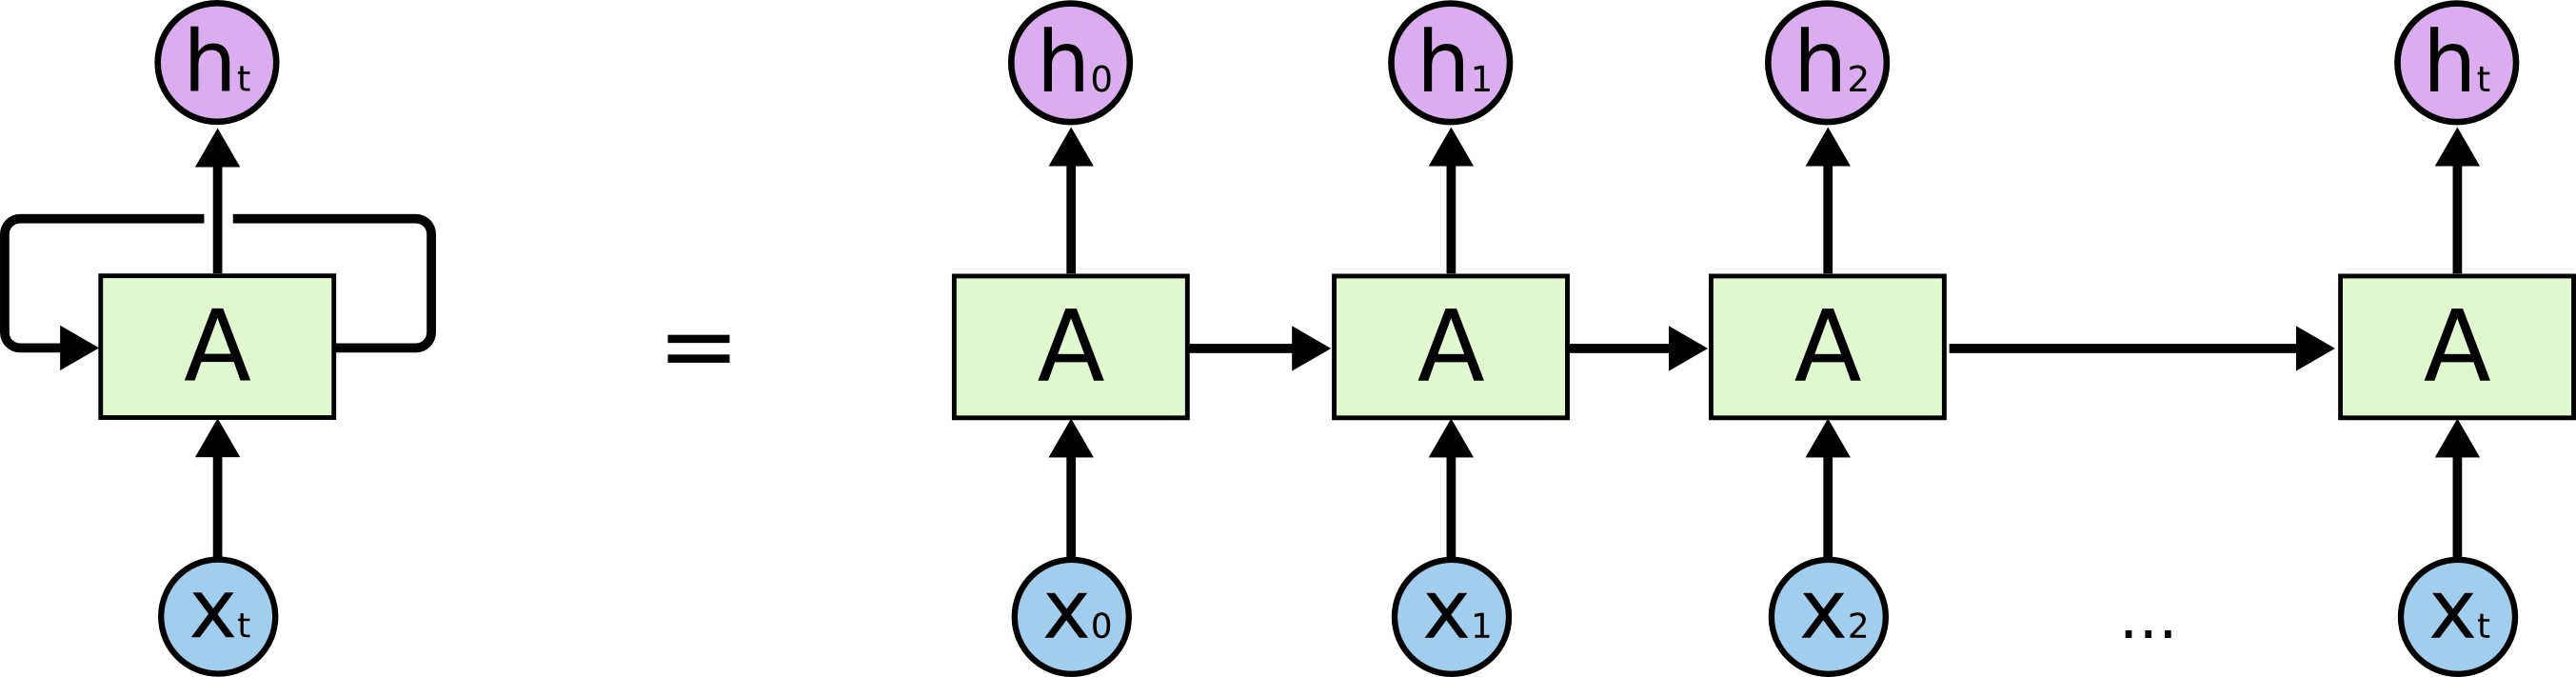
\includegraphics[width=\linewidth]{imgs/rnn_colah_unrolled.png}
\end{center}
\vspace{-15pt}
\captionof{figure}{Unrolled view of Recurrent Neural Network with Hidden States $h_i$ and inputs $x_i$. From \emph{Understanding LSTMs}, by Colah., 2015. \url{https://colah.github.io/posts/2015-08-Understanding-LSTMs/}. Copyright 2015 by Colah.}
%\vspace{15pt}
\label{fig:rnnUnrolledView}
\end{wrapfigure}


Traditional neural networks cannot persist information. As a comparison, while humans do not start thinking from scratch each time they learn something new, neural networks lack memory. Inherently related to sequences, recurrent neural networks use a recurrence or looping mechanism to introduce data persistence in the model to overcome this problem (Colah, 2015). This looping mechanism acts like a ``highway" to flow from one step to the next by passing inputs and modified hidden states along until computing a final prediction (Nguyen, 2018a). 

}



\subsubsection{Describing RNNs}

An RNN is a unidirectional \hyperref[sec:LanguageModels]{language model} since it uses context words left of the target word. It is a neural network that takes in a sequence (sentence) of input symbols (words) $\overrightarrow{x} = \{ x_1, ..., x_T\}$, and for each time $t$, the current hidden state $h_t$ is updated via the formula $h_t = f \Big( h_{t-1}, x_t \Big)$ where $f(\cdot)$ is a nonlinear activation function. The RNN's intermediate task is to predict a probability distribution over an input sequence (sentence) by predicting the next word symbol $x_t$ in the sequence sentence, using left context, so the output at time $t$ is the conditional distribution $P \Big(x_t \; | \; x_{t-1}, ..., x_1 \Big)$. The probability of the entire sequence sentence $\overrightarrow{x}$ is the product of all the probabilities of the individual words, $P(\overrightarrow{x}) = \prod_{t=1}^T P \Big(x_t \; | \; x_{t-1}, ..., x_1 \Big)$ (Cho, 2014). 


    
\subsection{Long-Short Term Memory Networks (LSTM)} \label{sec:LSTM}

\subsubsection{Motivation for LSTM: Vanishing Gradient Problem} \label{sec:ProblemWithRNNs}


{
\begin{wrapfigure}{L}{0.6\textwidth}
\begin{center}
    \vspace{-20pt}
    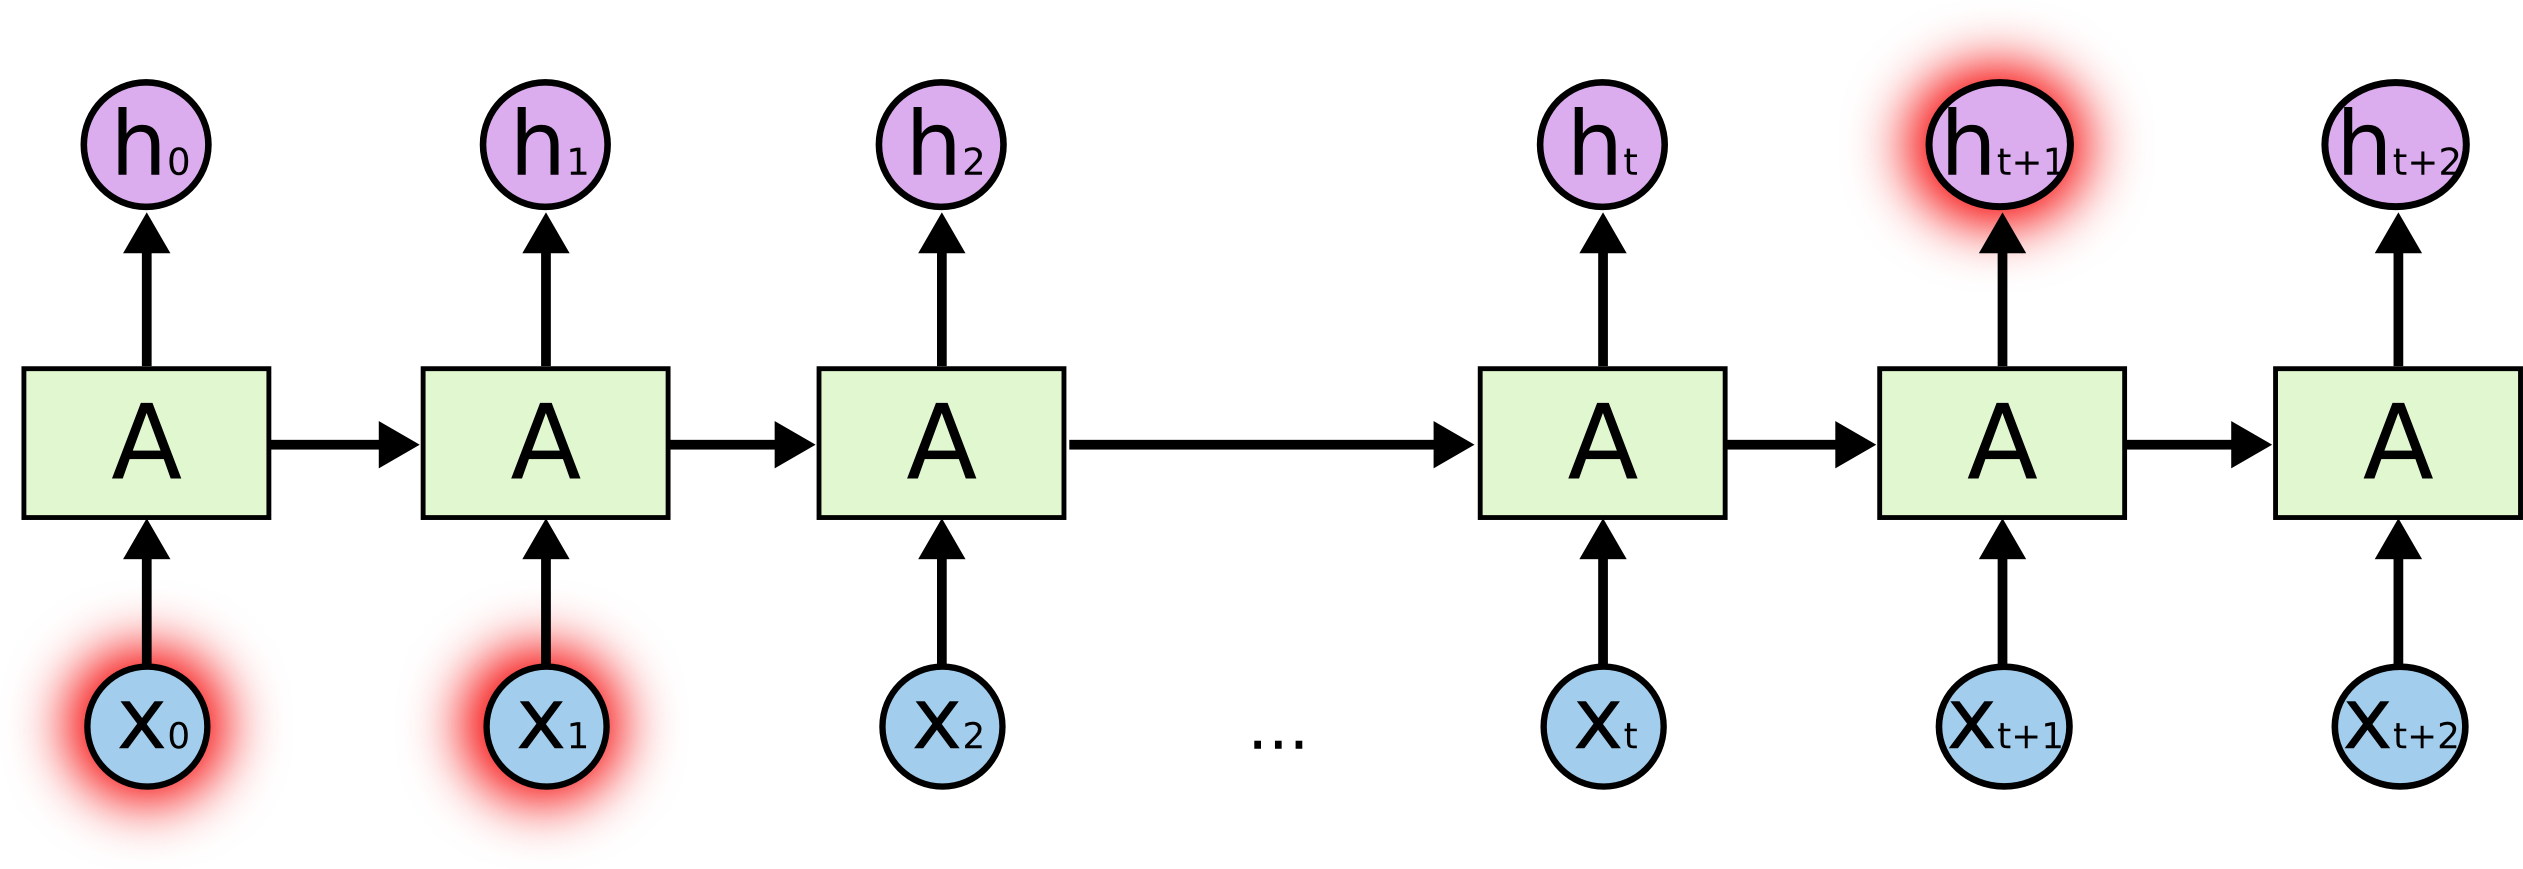
\includegraphics[width=\linewidth]{imgs/rnn_longterm.png}
\end{center}
\vspace{-15pt}
\captionof{figure}{Long-Term Dependency Problem in RNNs (widening gap between inputs $x_i$ and hidden states $h_j$. From \emph{Understanding LSTMs}, by Colah, 2015. \url{https://colah.github.io/posts/2015-08-Understanding-LSTMs/}. Copyright 2015 by Colah.}
%\vspace{15pt}
\label{fig:longTermMemoryProblem}
\end{wrapfigure}


\hyperref[sec:RNN]{RNN}s suffer from the well known \textbf{long-term dependency problem}. In some prediction tasks, longer context is needed to predict a target word. For instance to predict the last word in the sentence ``I grew up in France ... I speak fluent \emph{French}", a model would need the earlier context word ``France." When this gap between target and context words becomes too large, \hyperref[sec:RNN]{RNN}s cannot learn their relationship (Colah, 2015). 

Mathematically speaking, this is due to the \textbf{vanishing gradient problem}. During backward propagation of errors through the \hyperref[sec:RNN]{RNN}, the gradient shrinks as it back propagates through time and becomes too small to update the parameter weights significantly. 


}

This is compounded by the fact that since inputs at any timestep $t$ are dependent on previous $t-1$ outputs, longer sequences require more gradient calculations. Adjustments to earlier layers thus become smaller, causing gradients to shrink exponentially as they are backpropagated through to earlier layers of the \hyperref[sec:RNN]{RNN}. As a result, \hyperref[sec:RNN]{RNN}s ``forget" older history, resulting in short-term memory as shown in \cref{fig:longTermMemoryProblem} (Nguyen, 2018b). 



\subsubsection{Describing LSTMs}

A \textbf{long-short term memory network (LSTM)} is a type of \hyperref[sec:RNN]{RNN} that learns long-term dependencies by design, unlike \hyperref[sec:RNN]{RNN}s. LSTMs use gates or \hyperref[sec:NeuralLM]{neural network}s that decide how to add or remove information from the cell state, explicitly letting the LSTM ``remember" or ``forget" (Nguyen, 2018b). Since LSTMs can accumulate increasingly richer information while parsing the sentence, by the time the last word is reached, the hidden layer of the network provides a \textbf{semantic representation} of the entire sentence (Palangi et al., 2016). 

A core idea in an LSTM is the \textbf{cell state}, shown in \cref{fig:cellState} as the topmost line with the gates merging into it. For example, for a language predicting the next word based on previous ones, the appropriate behavior of its cell state might be to include the gender of the present subject so the model uses correct pronouns. When a new subject is observed, the cell state should forget the old subject's gender and retain the new one (Colah, 2015). 

From Nguyen (2018b), these gates regulate information flow as follows: 


% -------------------------------------------
% Start of the gates
\clearpage



%%% The forget gate image wrapping ---------------------
\begin{program}
\begin{wrapfigure}{L}{0.4\textwidth} 
\begin{center}
    \vspace{-30pt}
    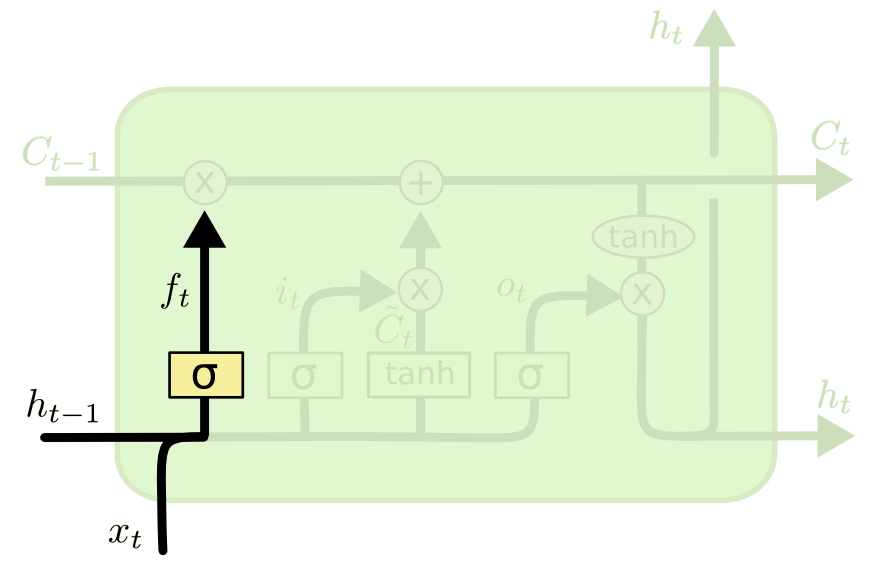
\includegraphics[width=0.9\linewidth]{imgs/lstm_forgetGate.png}
\end{center}
\captionof{figure}{ Forget Gate Calculation. From \emph{Understanding LSTMs}, by Colah, 2015. \url{https://colah.github.io/posts/2015-08-Understanding-LSTMs/}. Copyright 2015 by Colah.}
\label{fig:forgetGate}
\end{wrapfigure}

\ContentFontSize

\textbf{Forget Gate: } the forget gate, shown in \cref{fig:forgetGate}, decides information to discard or keep. The previous hidden state $h_{t-1}$ and current input $x_t$ are passed through the sigmoid nonlinearity function. The forget gate outputs a number between $0$ and $1$ for each number in the cell state $C_{t-1}$; values closer to $0$ indicate the forget gate should discard the information and values closer to $1$ should be kept. 

\begin{equation}
f_t = \sigma \Big( W_f \cdot [h_{t-1}, x_t] + b_f \Big)
\end{equation} 

where $f_t =$ forget gate for time $t$, $\sigma(\cdot) =$ sigmoid, $W_f =$ the weight matrix at the forget layer, and $b_f =$ forget gate's bias term. 

\end{program}



%%% The input gate image wrapping ---------------------
\begin{program}
\begin{wrapfigure}{L}{0.4\textwidth}
\begin{center}
    \vspace{-30pt}
    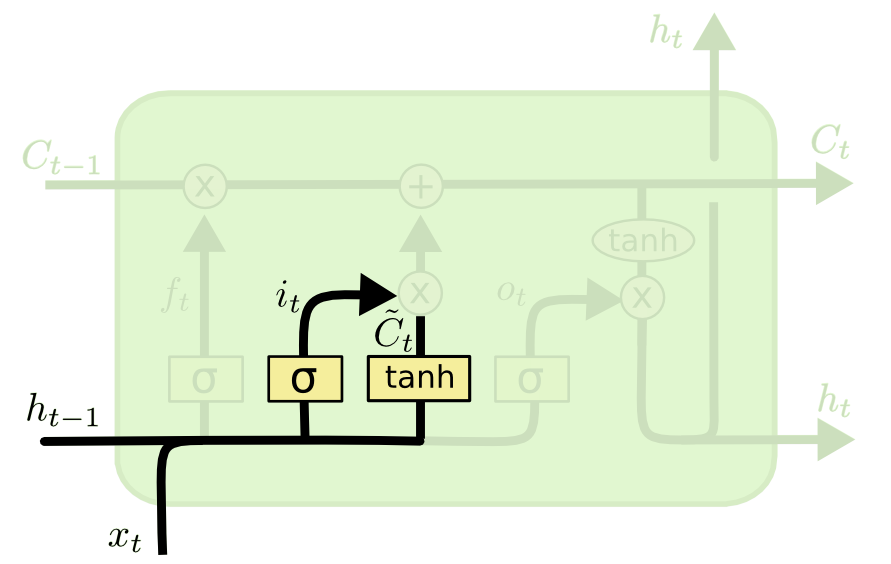
\includegraphics[width=0.9\linewidth]{imgs/lstm_inputGate.png}
\end{center}
\captionof{figure}{ Input Gate Calculation. From \emph{Understanding LSTMs}, by Colah, 2015. \url{https://colah.github.io/posts/2015-08-Understanding-LSTMs/}. Copyright 2015 by Colah.} 
\label{fig:inputGate}
\end{wrapfigure}

\ContentFontSize

\textbf{Input Gate: } the input gate $i_t$, shown in \cref{fig:inputGate}, updates the cell state $C_t$. Previous hidden state $h_{t-1}$ and current input $x_t$ are passed though a signmoid function normalize vector cells between $0$ and $1$. The input gate is later used with the cell state to decide how values are updated. 

\begin{equation}
i_t = \sigma \Big( W_i \cdot [h_{t-1}, x_t] + b_i \Big)
\end{equation}

where $i_t$ is the input gate for time $t$, $\sigma(\cdot)$ is the sigmoid, $W_i$ is the weight matrix at the input layer, and $b_i$ is the input gate's bias term. \par \kern 5pt
\end{program}





%%% The cell state gate image wrapping ---------------------
\begin{program}

\begin{wrapfigure}{L}{0.4\textwidth}
\begin{center}
    \vspace{-30pt}
    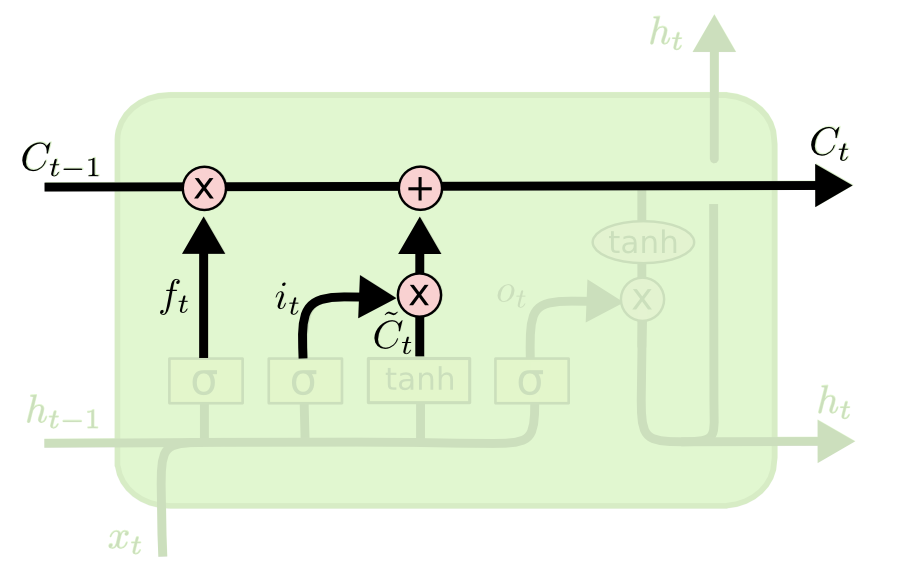
\includegraphics[width=0.9\linewidth]{lstm_cellState.png}    
\end{center}
%\vspace{-25pt}
\captionof{figure}{ Cell State Calculation. From \emph{Understanding LSTMs}, by Colah, 2015.\url{https://colah.github.io/posts/2015-08-Understanding-LSTMs/}. Copyright 2015 by Colah.}
\label{fig:cellState}
\end{wrapfigure}

\ContentFontSize

\textbf{Cell State: } Current cell state $C_t$, shown in \cref{fig:cellState}, takes $h_{t-1}$ and $x_t$ and normalizes them to be between $-1$ and $1$ via a hyperbolic tangent nonlinearity:

\begin{equation}
C_t = \tanh \Big( W_C \cdot [h_{t-1}, x_t] + b_C \Big)
\end{equation}

where $C_t$ is the cell state for time $t$, $\tanh(\cdot)$ is the hyperbolic tangent, $W_C$ is the weight matrix at the cell state layer, and $b_C$ is the cell state's bias term. Next, pointwise multiplications occur to regulate memory in LSTM: 

\begin{equation}
C_t = f_t \cdot C_{t-1} + i_t \cdot C_t
\end{equation}

\end{program}




%%% The output gate image wrapping ---------------------
\begin{program}
\begin{wrapfigure}{L}{0.4\textwidth}
\begin{center}
    \vspace{-30pt}
    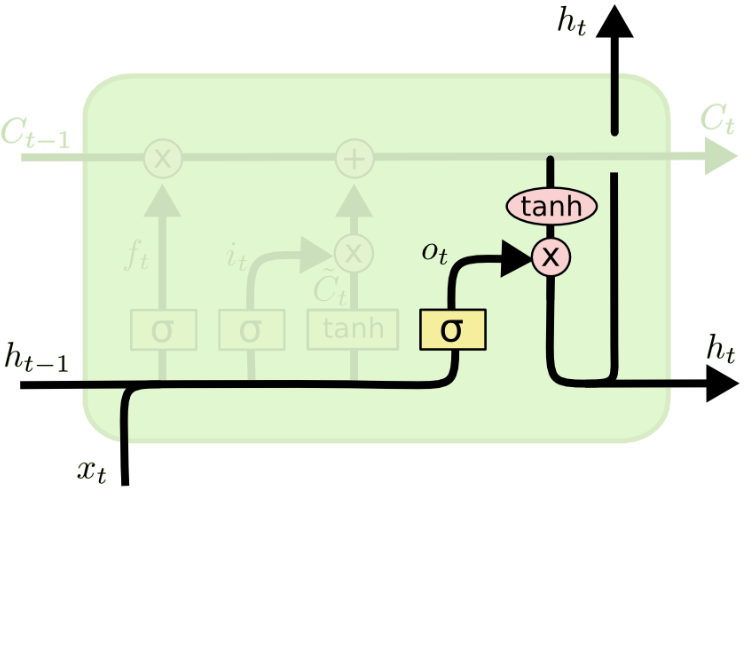
\includegraphics[width=0.27\textwidth]{imgs/lstm_outputGate.png}    
\end{center}
\captionof{figure}{Output Gate Calculation. From \emph{Understanding LSTMs}, by Colah, 2015.\url{https://colah.github.io/posts/2015-08-Understanding-LSTMs/}. Copyright 2015 by Colah.}
\label{fig:outputGate}
\end{wrapfigure}

\ContentFontSize

\textbf{Output Gate: }the output gate, shown in \cref{fig:outputGate}, determines the next hidden state by multiplying the previous output state by the cell state that is filtered by the hyperbolic tangent.

\begin{equation}
\begin{array}{ll}
o_t = \sigma \Big( W_o \cdot [h_{t-1}, x_t] + b_o \Big) \\
h_t = o_t \cdot \tanh(C_t)
\end{array}
\end{equation}

\end{program}


% End of the gates
\clearpage
% -------------------------------------------


\subsection{Gated Recurrent Networks (GRU)} \label{sec:GRU}

The gated recurrent unit (GRU) from Cho et al. (2014) is a type of LSTM that ``combines the forget and input gates into a single \textbf{update gate}" and ``merges the cell state and hidden state" (Colah, 2015), resulting with only the reset gate $r_t$ and update gate $z_t$ (Nguyen, 2018b). 

The \textbf{update gate} $z_t$ controls how much information from previous hidden state contributes to current hidden state, acting like a memory cell in the LSTM to remember long-term dependencies (Cho et al., 2014). 

The \textbf{reset gate} $r_t$ signals the hidden state on how to forget previous information. When the reset gate is close to $0$, the initialized hidden state $\Tilde{h}_t$ must ignore previous hidden state $h_{t-1}$ and reset with the current input $x_t$ only. Intuitively, this allows the activation hidden state $h_t$ to forget any irrelevant information for the future (Cho et al., 2014). 

\begin{figure}[h]
\vspace{-5pt}
\centering
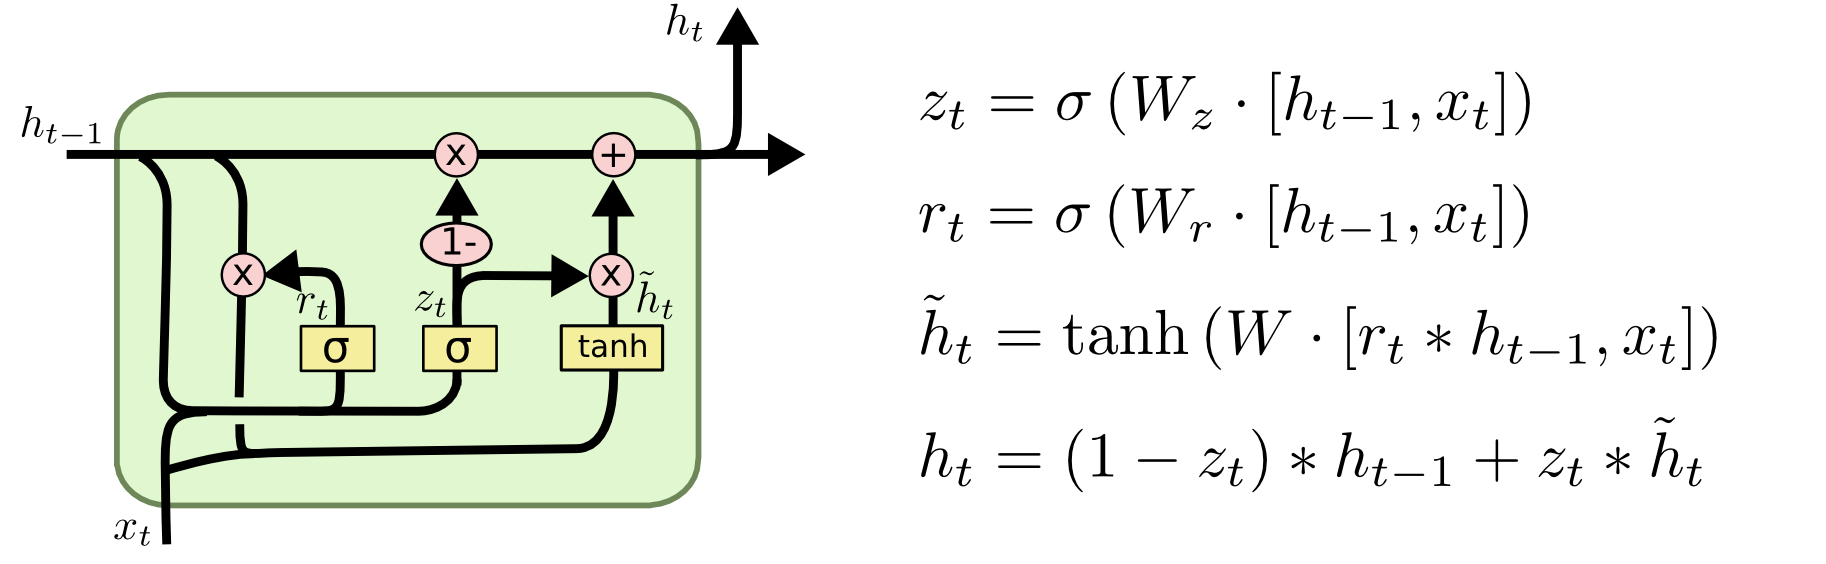
\includegraphics[width=0.8\textwidth]{imgs/gru_withformula.png}
\vspace{-5pt}
\caption{\footnotesize The GRU Cell with Gates. From \emph{Understanding LSTMs}, by Colah, 2015. \url{https://colah.github.io/posts/2015-08-Understanding-LSTMs/}. Copyright 2015 by Colah.}
\vspace{-5pt}
\label{fig:gru}
\end{figure}

Nguyen (2018b) notes that since GRU's have fewer tensor operations, they are more efficient than LSTMs during training. 
The GRU adaptively remembers and forgets because each hidden unit has separate reset and update gates so each hidden unit can capture dependencies over different time scales. Frequently active reset gates help the GRU remember short-term dependencies while frequently active update gates help the GRU note long-term dependencies (Cho et al., 2014). 

